\documentclass[a4paper,11pt]{article}
\usepackage[utf8x]{inputenc}      % input font encoding
\usepackage[lmargin=2.5cm,rmargin=2.5cm,tmargin=2.5cm,bmargin=3.5cm]{geometry}
\usepackage{amsmath,amssymb}
\usepackage[T1]{fontenc}          % output font encoding
\usepackage{booktabs,tabularx}
\usepackage{rotating}             % for sidewaystable
\usepackage[usenames]{xcolor}
\usepackage{tikz,tikz-uml}
\usepackage{listings}             % source code highlighting
\lstset{breaklines=true,
  breakatwhitespace=true,
  stepnumber=1,
  basicstyle=\ttfamily\footnotesize,
  commentstyle=\ttfamily\color{gray},
  prebreak={\textbackslash},
  breakindent=10pt,
  breakautoindent=false,
  showspaces=false,
  showstringspaces=false,
  frame=single}
\usepackage[pdftitle={FlexibleSUSY --- A spectrum generator generator for supersymmetric models},
pdfauthor={Jae-hyeon Park,Dominik Stockinger,Alexander Voigt},
pdfkeywords={FlexibleSUSY,supersymmetry,spectrum,generator,MSSM,NMSSM,E6SSM},
bookmarks=true, linktocpage]{hyperref}

\newcommand{\sarah}{\texttt{SARAH}}
\newcommand{\flexisusy}{\texttt{FlexibleSUSY}}

\newcommand{\code}[1]{\lstinline|#1|}  % inline source code
\newcommand{\textoverline}[1]{$\overline{\mbox{#1}}$}
\newcommand{\DRbar}{\textoverline{DR}}  % inline source code

\title{\bf FlexibleSUSY --- A spectrum generator generator for
  supersymmetric models}
\author{Jae-hyeon Park, Dominik St\"ockinger, Alexander Voigt\\[2em]
  {\sl Institut f\"ur Kern- und Teilchenphysik, TU Dresden, Dresden,
    Germany}}
\date{\today}

\begin{document}
\maketitle
\tableofcontents
\clearpage
\section{Overview}

Explain:
\begin{itemize}
\item What is FlexibleSUSY?
\item Features, design goals
\end{itemize}

\subsection{Requirements}

\begin{itemize}
\item Mathematica 7-9
\item SARAH version 4
\item a C++11 compatible compiler (g++ 4.7.2 or higher, clang++ 3.1 or
  higher)
\item a fortran compiler (gfortran etc.)
\item Eigen library version 3
\item Boost library
\item GNU scientific library
\item lapack (needed for the Lattice algorithm only)
\end{itemize}

\section{Quick start}
Create a MSSM spectrum generator
  \begin{lstlisting}[language=bash]
$ ./createmodel --models=MSSM
$ ./configure --with-models=MSSM
$ make
  \end{lstlisting}
Run the spectrum generator using the default parameter point
  \begin{lstlisting}[language=bash]
$ ./models/MSSM/run_MSSM.x
  \end{lstlisting}
Run the spectrum generator using a SLHA input file
  \begin{lstlisting}[language=bash]
$ ./models/MSSM/run_MSSM.x --slha-input-file=templates/MSSM/LesHouches.in.MSSM --slha-output-file=LesHouches.out.MSSM
  \end{lstlisting}

\section{Usage}
\subsection{Files and directories}

Explain:
\begin{itemize}
\item Soucre code directories and files
\item Model directories and files
\end{itemize}

\subsection{Basic commands}

Explain:
\begin{itemize}
\item ./createmodel
\item ./configure
\item make
\item Mathematica interface (see models/<model>/start.m)
\end{itemize}

\subsection{Model files}

Explain how to write a FlexibleSUSY model file (starting from a SARAH
model file).

A FlexibleSUSY model file is a Mathematica file, where the following
pieces are defined:

\paragraph{General model information}

\subparagraph{FSModelName}
Name of the FlexibleSUSY model.
Example (MSSM):
\begin{lstlisting}[language=Mathematica]
FSModelName = "MSSM";
\end{lstlisting}

\subparagraph{OnlyLowEnergyFlexibleSUSY} If set to True, creates a
spectrum generator without high-scale constraint, i.e.\ only a
low-scale and susy-scale constraint will be created (default: False).
In this case all model parameters, except for gauge and Yukawa
couplings are input at the susy scale.  This option is similar to
\texttt{OnlyLowEnergySPheno} in SARAH/SPheno.
\\
Example:
\begin{lstlisting}[language=Mathematica]
OnlyLowEnergyFlexibleSUSY = False;  (* default *)
\end{lstlisting}

\paragraph{Input and output parameters}

\subparagraph{MINPAR} This list of two-component lists defines model
input parameters and their SLHA keys.  These parameters will be read
from the MINPAR block in the SLHA file.
\\
Example (MSSM):
\begin{lstlisting}[language=Mathematica]
MINPAR = { {1, m0},
           {2, m12},
           {3, TanBeta},
           {4, Sign[\[Mu]]},
           {5, Azero}
         };
\end{lstlisting}

\subparagraph{EXPAR} This list of two-component lists defines further
model input parameters and their SLHA keys.  These parameters will be
read from the EXTPAR block in the SLHA file.
\\
Example (E6SSM):
\begin{lstlisting}[language=Mathematica]
EXTPAR = { {61, LambdaInput},
           {62, KappaInput},
           {63, muPrimeInput},
           {64, BmuPrimeInput},
           {65, vSInput}
         };
\end{lstlisting}

\subparagraph{DefaultParameterPoint} This list of two-component lists
defines default values for the model input parameters.
\\
Example (MSSM):
\begin{lstlisting}[language=Mathematica]
DefaultParameterPoint = {
    {m0, 125},
    {m12, 500},
    {TanBeta, 10},
    {Sign[\[Mu]], 1},
    {Azero, 0}
};
\end{lstlisting}

\paragraph{Constraints}
Currently three constraints are supported: low-scale, susy-scale and
high-scale constraints.  In FlexibleSUSY they are named as
\texttt{LowScale}, \texttt{SUSYScale} and \texttt{HighScale}.  For
each constraint there is a scale definition (named after the
constraint), an initial guess for the scale (concatenation of the
constraint name and \texttt{FirstGuess}) and a list settings to be
applied at the constraint (concatenation of the constraint name and
\texttt{Input}).
\\
Example (MSSM):
\begin{lstlisting}[language=Mathematica]
(* susy-scale constraint *)
SUSYScale = Sqrt[M[Su[1]]*M[Su[6]]];        (* scale definition *)
SUSYScaleFirstGuess = Sqrt[m0^2 + 4 m12^2]; (* first scale guess *)
SUSYScaleInput = {};                        (* nothing is set here *)

(* high-scale constraint *)
HighScale = g1 == g2;                       (* scale definition *)
HighScaleFirstGuess = 1.0 10^14;            (* first scale guess *)
HighScaleInput = {
   {T[Ye], Azero*Ye},
   {T[Yd], Azero*Yd},
   {T[Yu], Azero*Yu},
   {mHd2, m0^2},
   {mHu2, m0^2},
   {mq2, UNITMATRIX[3] m0^2},
   {ml2, UNITMATRIX[3] m0^2},
   {md2, UNITMATRIX[3] m0^2},
   {mu2, UNITMATRIX[3] m0^2},
   {me2, UNITMATRIX[3] m0^2},
   {MassB, m12},
   {MassWB,m12},
   {MassG, m12}
};

LowScale = SM[MZ];                          (* scale definition *)
LowScaleFirstGuess = SM[MZ];                (* first scale guess *)
LowScaleInput = {
   {vd, 2 MZDRbar / Sqrt[GUTNormalization[g1]^2 g1^2 + g2^2] Cos[ArcTan[TanBeta]]},
   {vu, 2 MZDRbar / Sqrt[GUTNormalization[g1]^2 g1^2 + g2^2] Sin[ArcTan[TanBeta]]}
};
\end{lstlisting}

\paragraph{Initial parameter guesses} At the \texttt{LowScale} and
\texttt{HighScale} it is recommended to make an initial guess for the
model parameters.  This can be done via
\begin{lstlisting}[language=Mathematica]
InitialGuessAtLowScale = {
   {vd, SM[vev] Cos[ArcTan[TanBeta]]},
   {vu, SM[vev] Sin[ArcTan[TanBeta]]}
};

InitialGuessAtHighScale = {
   {\[Mu]   , 1.0},
   {B[\[Mu]], 0.0}
};
\end{lstlisting}

\begin{sidewaystable}[tb]
  \centering
  \begin{tabularx}{\textwidth}{>{\ttfamily}l>{\ttfamily}lX}
    \toprule
    variable    & default value & description \\
    \midrule
    FSModelName & Model`Name & Name of the FlexibleSUSY model \\
    OnlyLowEnergyFlexibleSUSY & False & low-energy model \\
    MINPAR & \{\} & list of input parameters in SLHA MINPAR block \\
    EXTPAR & \{\} & list of input parameters in SLHA EXTPAR block \\
    DefaultParameterPoint & \{\} & list of default values for the input parameters \\
    LowScale & SM[MZ] & Standard Model matching scale (in GeV) \\
    LowScaleFirstGuess & SM[MZ] & first guess for the Standard Model matching scale (in GeV) \\
    LowScaleInput & \{\} & settings applied at the low scale \\
    SUSYScale & 1000 & scale of supersymmetric particle masses (in GeV) \\
    SUSYScaleFirstGuess & 1000 & first guess for the susy scale (in GeV) \\
    SUSYScaleInput & \{\} & settings applied at the susy scale \\
    HighScale & SARAH`hyperchargeCoupling == SARAH`leftCoupling
      & unification scale (in GeV) \\
    HighScaleFirstGuess & $10^{14}$ & first guess for the unification scale (in GeV) \\
    HighScaleInput & \{\} & settings applied at the unification scale \\
    \bottomrule
  \end{tabularx}
  \caption{FlexibleSUSY model file variables}
  \label{tab:model-file-variables}
\end{sidewaystable}

\subsection{Makefile modules}

Explain how to write a custom makefile module (module.mk) for a
FlexibleSUSY model.

\section{Output}
\subsection{Files}

Explain the created C++ files and executables, and how to use them.

\subsection{Two-scale algorithm}

Explain the structure of the two-scale algorithm classes and how they
work and are plugged together.


The stucture of the two-scale algorithm used in \flexisusy\ is as follows,%

Initial guess:
\begin{enumerate}
\item Guess gauge couplings $g_{1,2,3}$ at $m_Z$
\item Apply user-defined low-scale constraint (\code{LowScaleInput})
\item Guess Yukawa couplings $y^{u,d,e}_{ij}$ at $m_Z$
\item Run model to the high-scale (\code{HighScaleFirstGuess})
\item Apply high-scale constraint (\code{HighScaleInput})
\item Run model to the low-scale (\code{LowScaleFirstGuess})
\item Solve EWSB eqs.\ at the tree-level
\item Calculate \DRbar\ masses
\end{enumerate}
%
Solving the renormalization group equations:
\begin{enumerate}
\item \label{rge-step-one} Run model to the low-scale (\code{LowScale})
  \begin{enumerate}
  \item Calculate \DRbar\ masses
  \item Recalculate low-scale
  \item Calculate \DRbar\ gauge and Yukawa couplings $g_{1,2,3}$,
    $y^{u,d,e}_{ij}$, see
    Section~\ref{sec:matching-to-the-standard-model}.
  \item Apply user-defined low-scale constraint (\code{LowScaleInput})
  \end{enumerate}
\item Run model to the high-scale (\code{HighScale})
  \begin{enumerate}
  \item Recalculate high-scale
  \item Apply high-scale constraint (\code{HighScaleInput})
  \end{enumerate}
\item Run model to the susy-scale (\code{SUSYScale})
  \begin{enumerate}
  \item Calculate \DRbar\ masses
  \item Recalculate low-scale
  \item Apply susy-scale constraint (\code{SUSYScaleInput})
  \item Solve EWSB eqs.\ at the one-loop level
  \end{enumerate}
\item If not converged yet, goto \ref{rge-step-one}
\end{enumerate}
%
Calculating the particle spectrum:
\begin{enumerate}
\item Run model to the susy-scale
\item Calculate the pole masses
\item Run model to the parameter output scale (SLHA block MODSEL 12)
\end{enumerate}

\begin{figure}[tb]
  \centering
  \tikzumlset{fill class=white}
  \begin{tikzpicture}
    \umlclass[x=0, y=0, type=abstract]{Beta\_function}{
      -- scale : double\\
      -- loops : unsigned\\
      -- numPars : unsigned
    }{
      + \umlvirt{display() : const Eigen::ArrayXd} \\
      + \umlvirt{set(v : const Eigen::ArrayXd\&) : void}\\
      + \umlvirt{beta() : Eigen::ArrayXd}\\
      + run\_to(scale : double, eps : double) : void\\
    }
    \umlclass[x=8, y=-12, template={T}]{MSSM}{}{}
    \umlclass[x=8, y=-8, type=abstract]{Two\_scale\_model}{}{
      + \umlvirt{calculate\_spectrum() : void}\\
      + \umlvirt{run\_to(scale : double, eps : double) : void}\\
      + \umlvirt{set\_precision(precision : double) : void}
    }
    \umlclass[x=0, y=-4]{MSSM\_susy\_parameters}{}{
      + display() : const Eigen::ArrayXd \\
      + set(v : const Eigen::ArrayXd\&) : void\\
      + beta() : Eigen::ArrayXd
    }
    \umlclass[x=0, y=-8]{MSSM\_soft\_parameters}{}{
      + display() : const Eigen::ArrayXd \\
      + set(v : const Eigen::ArrayXd\&) : void\\
      + beta() : Eigen::ArrayXd
    }
    \umlclass[x=0, y=-12]{MSSM$<$Two\_scale$>$}{}{
      + calculate\_spectrum() : void\\
      + run\_to(scale : double, eps : double) : void\\
      + set\_precision(precision : double) : void
    }
   \umlinherit{MSSM\_susy\_parameters}{Beta\_function}
   \umlinherit{MSSM\_soft\_parameters}{MSSM\_susy\_parameters}
   \umlinherit{MSSM$<$Two\_scale$>$}{MSSM\_soft\_parameters}
   \umlinherit{MSSM$<$Two\_scale$>$}{Two\_scale\_model}
   \umldep[arg1={$<<$bind$>>$}, mult1={T $\rightarrow$ Two\_scale}, pos1=0.5]{MSSM$<$Two\_scale$>$}{MSSM}
  \end{tikzpicture}
  \caption{Two-scale model class hierarchy}
  \label{fig:two-scale-model-class-hierarchy}
\end{figure}

\begin{figure}[tb]
  \centering
  \tikzumlset{fill class=white}
  \begin{tikzpicture}
    \umlclass[x=0, y=0, type=abstract]{Two\_scale\_model}{}{
      + \umlvirt{calculate\_spectrum() : void}\\
      + \umlvirt{run\_to(scale : double, eps : double) : void}\\
      + \umlvirt{set\_precision(precision : double) : void}
    }
    \umlclass[x=0, y=-4]{RGFlow$<$Two\_scale$>$}{}{
      + solve() : void
    }
    \umlclass[x=8, y=0]{Constraint$<$Two\_scale$>$}{}{
      + \umlvirt{apply() : void}\\
      + \umlvirt{get\_scale() : double}\\
      + \umlvirt{set\_model(model : Two\_scale\_model*) : void}
    }
    \umlclass[x=8, y=4, template={T}]{Constraint}{}{}
    \umlclass[x=0, y=-7]{Initial\_guesser$<$Two\_scale$>$}{}{
      + \umlvirt{guess() : void}
    }
    \umlclass[x=0, y=-11, template={T}]{Initial\_guesser}{}{}
    \umlclass[x=8, y=-7]{Convergence\_tester$<$Two\_scale$>$}{}{
      + \umlvirt{accuracy\_goal\_reached() : bool}\\
      + \umlvirt{max\_iterations() : unsigned}
    }
    \umlclass[x=8, y=-11, template={T}]{Convergence\_tester}{}{}
    \umlclass[x=8, y=-4, template={T}]{RGFlow}{}{}
    \umldep[arg1={$<<$bind$>>$}, mult1={T $\rightarrow$ Two\_scale}, pos1=0.5]{RGFlow$<$Two\_scale$>$}{RGFlow}
    \umldep[mult1=1..*]{RGFlow$<$Two\_scale$>$}{Two\_scale\_model}
    \umldep[mult1=1..*]{RGFlow$<$Two\_scale$>$}{Constraint$<$Two\_scale$>$}
    \umldep{RGFlow$<$Two\_scale$>$}{Initial\_guesser$<$Two\_scale$>$}
    \umldep{RGFlow$<$Two\_scale$>$}{Convergence\_tester$<$Two\_scale$>$}
    \umldep[mult1={$<<$bind$>>$}, arg1={T $\rightarrow$ Two\_scale}, pos1=0.5]{Initial\_guesser$<$Two\_scale$>$}{Initial\_guesser}
    \umldep[mult1={$<<$bind$>>$}, arg1={T $\rightarrow$ Two\_scale}, pos1=0.5]{Convergence\_tester$<$Two\_scale$>$}{Convergence\_tester}
    \umldep[arg1={$<<$bind$>>$}, mult1={T $\rightarrow$ Two\_scale}, pos1=0.5]{Constraint$<$Two\_scale$>$}{Constraint}
  \end{tikzpicture}
  \caption{Two-scale renormalization group solver class hierarchy}
  \label{fig:two-scale-rgflow-class-hierarchy}
\end{figure}

\subsubsection{Matching to the Standard Model}
\label{sec:matching-to-the-standard-model}

At the low-scale $M_Z$ we calculate
%
\begin{align}
  \alpha_{\text{e.m.},\text{susy}}^{\text{\DRbar}}(M_Z) &=
  \frac{\alpha_{\text{e.m.},\text{SM}}^{(5),\text{\MSbar}}(M_Z)}{1 -
    \Delta\alpha_{\text{e.m.},\text{SM}}(M_Z) -
    \Delta\alpha_{\text{e.m.},\text{susy}}(M_Z)} ,\\
  \Delta\alpha_{\text{e.m.},\text{SM}}(\mu) &=
  \frac{\alpha_\text{e.m.}}{2\pi} \left[\frac{1}{3}
    - \frac{16}{9} \log{\frac{m_t}{\mu}} \right],\\
  \Delta\alpha_{\text{e.m.},\text{susy}}(\mu) &=
  \frac{\alpha_\text{e.m.}}{2\pi} \left[ -\sum_{\text{susy particle }
      i}
    C_i \log{\frac{m_i}{\mu}} \right],\\
    e_{\text{susy}}^{\text{\DRbar}}(M_Z) &=
    \sqrt{4\pi\alpha_{\text{e.m.},\text{susy}}^{\text{\DRbar}}(M_Z)}
\end{align}
%
\begin{align}
  \alpha_{\text{s},\text{susy}}^{\text{\DRbar}}(M_Z) &=
  \frac{\alpha_{\text{s},\text{SM}}^{(5),\text{\MSbar}}(M_Z)}{1 -
    \Delta\alpha_{\text{s},\text{SM}}(M_Z)
    - \Delta\alpha_{\text{s},\text{susy}}(M_Z)} ,\\
  \Delta\alpha_{\text{s},\text{SM}}(\mu) &=
  \frac{\alpha_\text{s}}{2\pi} \left[
    -\frac{2}{3} \log{\frac{m_t}{\mu}} \right],\\
  \Delta\alpha_{\text{s},\text{susy}}(\mu) &=
  \frac{\alpha_\text{s}}{2\pi}\left[ \frac{1}{2}-\sum_{\text{susy
        particle } i} C_i \log{\frac{m_i}{\mu}} \right]
\end{align}
%

\subsection{Lattice algorithm}

Explain the structure of the lattice algorithm classes and how they
work.


\end{document}
